% Generated by tools/generate_statements_only_paper.py.
% Do not edit this derived file; edit the canonical paper source instead.

\subsection{Nonsupercritical, T3-like, and Vd1/Vd2 Reach Branches}
\label{sec:t3-vd-demand-branches}

\subsubsection{The exactly-one-$T3$ branch}

\begin{proposition}[Exactly one T3-like V triangle]
\label{prop:nplus-one-one-t3}
Assume the C triangle is CE1 or CE2, $N_+=1$, exactly one V triangle is
T3-like, and no triangle is Vd1 or Vd2.  Then the triangles do not cover $H$.
\end{proposition}

% Proof environment omitted (source: 04e_strategy2_verification_04_nonsupercritical_t3_like_and_vd1_vd2_demand_branches.tex).

\subsubsection{The nonsupercritical CE1/CE2 boundary packages}

Figure~\ref{fig:ce1-ce2-n0-all-vd0} gives a common schematic for the package
recorded below.

\begin{figure}[H]
\centering
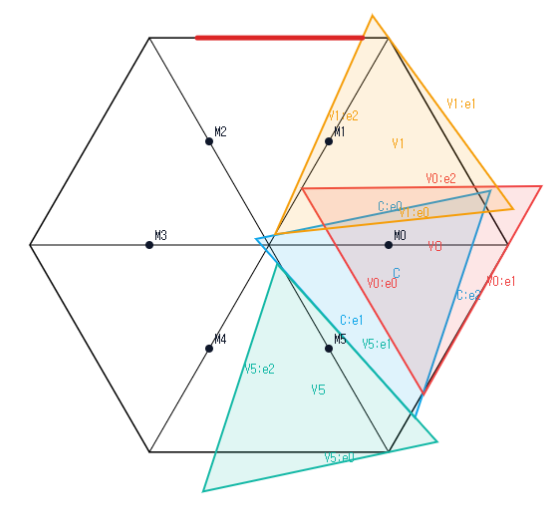
\includegraphics[width=.78\linewidth]
  {figures/strategy2_ce1_ce2_n0_all_vd0.png}
\caption{Schematic view of the common CE1/CE2, $N_+=0$, all-Vd0 boundary
package, not to scale.  The C triangle and three representative Vd0 vertex
triangles are shown; the remaining three triangles are omitted for
readability.  The simultaneous placement is not a candidate cover, and no
conclusion depends on visual inspection.}
\label{fig:ce1-ce2-n0-all-vd0}
\end{figure}

\begin{proposition}[All-Vd0 skeleton-data obstruction]
\label{prop:nplus-zero-all-vd0}
Let the C triangle be CE1 or CE2. Assume all six V triangles are Vd0,
\[
 A_i+B_i\le1\qquad(i=0,\ldots,5),
\]
and the seven open triangles cover the full skeleton
\[
 S=\partial H\cup\bigcup_{i=0}^5r_i.
\]
Then no such configuration exists. Consequently the same distinguished-index data cannot
cover all of $H$.
\end{proposition}

% Proof environment omitted (source: 04e_strategy2_verification_04_nonsupercritical_t3_like_and_vd1_vd2_demand_branches.tex).

We next treat the additional T3-like V triangles in the $N_+=0$ branch.  The
following local facts also reappear later.

\begin{lemma}[T3-like midpoint and side tradeoff]
\label{lem:t3-midpoint-tradeoff}
Let $T_i$ be T3-like.  Then $M_i\notin T_i$.  After applying the closed-trace
domination of Proposition~\ref{prop:t3-translation}, suppose
$\Haus(T_i\cap r_{i+1})>0$ and $M_{i+1}$ belongs to the dominated trace.
If $b$ is its boundary reach toward $V_{i+1}$, $c$ its exit on $r_i$, and
$\ell$ its entry on $r_{i+1}$, all measured from the relevant
vertex, then
\begin{equation}
 b+c<1,\qquad b+\ell>1.
 \label{eq:t3-side-tradeoff}
\end{equation}
Consequently two T3-like traces $T_i,T_{i+1}$ that cover each other's
midpoint, with positive traces on $r_{i+1}$ and $r_i$, respectively, cannot
cover both segments $[V_i,M_i]$ and $[V_{i+1},M_{i+1}]$ if no other triangle
has positive trace there.
\end{lemma}

% Proof environment omitted (source: 04e_strategy2_verification_04_nonsupercritical_t3_like_and_vd1_vd2_demand_branches.tex).

\begin{lemma}[The support-isolated four-branch inequality]
\label{lem:407-four-label-loss}
\label{thm:s2-geom-t3}
Assume the support-isolated T3-like endpoint state of
Definition~\ref{def:body-t3-endpoint-state}.  Then the two endpoint V triangles
satisfy
\begin{equation}
 \overline M_{c_5^\ast}(a_5^\ast)+\overline M_{c_1^\ast}(a_1^\ast)<1,
 \label{eq:407-loss}
\end{equation}
where $a_1^\ast,a_5^\ast$ are the exact boundary inputs and
$c_1^\ast,c_5^\ast$ the exact radial lower bounds defined there.
\end{lemma}

% Proof environment omitted (source: 04e_strategy2_verification_04_nonsupercritical_t3_like_and_vd1_vd2_demand_branches.tex).

\begin{proposition}[The $N_+=0$ T3-like branch]
\label{prop:nplus-zero-t3}
Assume that $T_C$ is CE1 or CE2, $N_+=0$, no V triangle is Vd1 or Vd2,
and at least one V triangle is T3-like.  Then the seven triangles do not cover
$H$.
\end{proposition}

% Proof environment omitted (source: 04e_strategy2_verification_04_nonsupercritical_t3_like_and_vd1_vd2_demand_branches.tex).

\subsubsection{Two reusable high-radial endpoint inequalities}

\begin{lemma}[One-side endpoint loss]
\label{lem:one-side-capped-loss}
\label{thm:s2-geom-e1}
Let $0<R<1$, $S=\sqrt{1-R+R^2}$, and let $s,u,w>0$ satisfy
$s+u+w=1$ and $0<u<R$.  Put
\[
 \delta=\frac{R}{1+S},\qquad
 \gamma=u-\delta-\frac{R}{1-R}w,
\]
and assume $\gamma>0$.  Set
\[
 c_1=u/R,\qquad c_5=1-\gamma.
\]
Then
\begin{equation}
 \overline M_{c_5}(s)+\overline M_{c_1}(u)<1.
 \label{eq:one-side-loss}
\end{equation}
\end{lemma}

% Proof environment omitted (source: 04e_strategy2_verification_04_nonsupercritical_t3_like_and_vd1_vd2_demand_branches.tex).

\begin{lemma}[CE2 two-endpoint loss]
\label{lem:two-endpoint-capped-loss}
\label{thm:s2-geom-e2}
Let $[x,U]$ and $[y,v]$ be the two exact CE2 traces in the legacy
coordinates of Remark~\ref{rem:signed-legacy-variables}, where $U$ denotes
the endpoint called $u$ there.  Put
\[
 p=1-U,\qquad q=1-v,\qquad
 r=\frac{x}{x+y},\qquad w=\frac{y}{x+y},
\]
and reflect if necessary so that $0<w\le1/2$ and $r=1-w$.  Then
\begin{equation}
 \overline M_{p/w}(p)+\overline M_{q/r}(q)<1.
 \label{eq:two-endpoint-loss}
\end{equation}
\end{lemma}

% Proof environment omitted (source: 04e_strategy2_verification_04_nonsupercritical_t3_like_and_vd1_vd2_demand_branches.tex).

\subsubsection{The exactly-one-Vd1/Vd2 placements}

We now assume CE2, $N_+=1$, and exactly one V triangle is Vd1 or Vd2.  The corner
normal form of Proposition~\ref{prop:vd-corner-normal-form} will be used in
the following form: for some $t>0$ and $d=\sqrt{t^2+t+1}$,
\begin{equation}
 x-(t+1)y\le a,\qquad ty-(t+1)x\le tb,\qquad
 tx+y\le d-a-tb.
 \label{eq:vd-corner-form}
\end{equation}
In particular $a+b<1/2$ for the Vd1/Vd2 triangle in this corner normal
form.

\begin{lemma}[Vd1 adjacent rescue]
\label{lem:vd1-adjacent-rescue}
Assume an original open-triangle skeleton cover in the CE2 branch with
$T_C\cap\{M_0,\ldots,M_5\}=\{M_0\}$,
with $T_0$ the unique Vd1 V triangle, $M_1\in T_0$, $T_1$ uniquely supercritical,
$T_2,\ldots,T_5$ nonsupercritical Vd0, and
\[
 \Haus(T_i\cap r_{i-1})=\Haus(T_i\cap r_{i+1})=0
 \qquad(i=1,\ldots,5).
\]
Then the perimeter together with $r_1$ is not covered.
\end{lemma}

% Proof environment omitted (source: 04e_strategy2_verification_04_nonsupercritical_t3_like_and_vd1_vd2_demand_branches.tex).

\begin{lemma}[Vd1-pair replacement interface]
\label{lem:vd1-pair-replacement}
In the remaining adjacent Vd1--supercritical placement, the pair can be
replaced by two open nonsupercritical Vd0 triangles while preserving full skeleton
coverage.
\end{lemma}

% Proof environment omitted (source: 04e_strategy2_verification_04_nonsupercritical_t3_like_and_vd1_vd2_demand_branches.tex).

\subsubsection{Final boundary-propagation cases}

\begin{proposition}[Cases excluded by boundary propagation]
\label{prop:demand-branches}
Boundary-reach propagation gives the following exclusions:
\begin{enumerate}
\item CE1 or CE2, $N_+=0$, all V triangles Vd0;
\item CE1 or CE2, $N_+=0$, with at least one T3-like triangle and no Vd1/Vd2;
\item CE1 or CE2, $N_+=1$, all V triangles Vd0, with at least one boundary
gap;
\item CE1 or CE2, $N_+=1$, exactly one T3-like triangle and no Vd1/Vd2;
\item the CE2, $N_+=1$, exactly-one-Vd1/Vd2 branch with no T3-like
triangle.
\end{enumerate}
All gap alternatives include singleton gaps.
\end{proposition}

% Proof environment omitted (source: 04e_strategy2_verification_04_nonsupercritical_t3_like_and_vd1_vd2_demand_branches.tex).

% ---- Complete 407X case analysis and two-chart replacement ----
